\documentclass[../main.tex]{subfiles}

\begin{document}

\section{WASM}
\subsection{Definitions}
(\href{https://webassembly.github.io/spec/core/}{wasm-core})
(\href{}{wasm-polkadot})
(\href{https://www.ngzhian.com/relaxed-simd/core/_download/WebAssembly.pdf}{wasm-spec})

WebAssembly, shortened to Wasm, is a binary instruction format for a stack-based virtual machine ~\cite{wasm-core-spec}. It is a platform-agnostic binary format, meaning it will run the exact instructions across whatever machine it operates on. ~\cite{wasm-polkadot-wiki}

`asm.js` was Wasm precursor, but browser vendors like Mozilla, Google, Microsoft, and Apple focused on the Wasm design. The main goal was to create a binary format with some mandatory features: compact, support for streaming complication and sanboxed execution.

Wasm is currently a compilation target for a lot of high level language, this allows languages to enter the web-world, in client or server side, but also in completely different applications.

Examples are plugins, applications are able to accept, execute and make the wasm code to interact with the environment, allowing different High-Level languages to work together having wasm as minimum common divisor.

The main design goals in the wasm specification introduction ~\cite{wasm-core-spec} are:
\begin{description}[font=$\bullet$ \scshape\bfseries]
  \item[Fast] It's design allow to create executor with so less overhead that the execution is almost fast as native code
  \item[Safe] It is completely memory-safe as long as the executor is correctly behaving, sandboxing the execution properly
  \item[Well-defined] The definition of the binary format makes easy to create a valid executor that makes the code behave correctly
  \item[Hardware-independent] The compilation process is independent by the architecture that will run the code
  \item[Language-independent] There's no strong influence by other binary format, language or programming model
  \item[Platform-independent] It can be compiled and be executed on all modern architectures, embedded systems or applications as browsers
  \item[Open] There is simple way to interoperate the with executor/environment
\end{description}

Other important considerations are made on the efficiency and portability, the specification describe wasm also as: compact, modular, efficient, streamable, and parallelizable.

% Something not clear at first look is \"modular\", it means that the program can be split into smaller parts and those can be transmitted, cahed and consumed separately.

In the following chapters the words executor or embedder have the same meaning.

\subsection{Specifications}

The specification does not make any assumption on the embedder, this makes it completely constraint-less, it just must follows all the defined instruction set, binary encoding, validation, and execution semantics ~\cite{wasm-core-spec}.

Wasm is stack-based, this means that the instruction set is very different from the standards architecture's bytecode that normally are registered-based. Wasm has also a one-to-one text representation other than the normal binary representation, of course it makes the code less compact but almost human readable.

All the concepts present in the specifications are very high-level even if it is a low level language, some of them are:

%\begin{description} [style=nextline]
\begin{description}[font=$\bullet$ \scshape\bfseries]
  \item[Values]
        Wasm has only four data type, integers and floating points (following IEEE 754 standard) both 32 and 64 bits
  \item[Instructions]
        Being a stack based language every instruction works implicit on a stack but there is a general division between:
        \begin{itemize}
          \item Simple Instructions, performing basic operations on data
          \item Control Flow, allowing to follow some high-level language control flow having nested blocks
        \end{itemize}
  \item[Traps]
        Those are instructions which immediately aborts the execution, the termination is not handled by wams itself but by the embedder
  \item[Functions]
        Being so new, this assembly-like language, allow users to work with functions abstracting some standards assembly's complexity
  \item[Linear Memory]
        This is where the communication between the code and the environment happens, like the name says this is a contiguous area of memory given to the code. This memory is very crucial for the security considerations that we will see later.
  \item[Modules]
        A Module contains everything just explained, this is the logical container of the code. Every wasm code is made by a single module.
  \item[Exports] Once the module is instantiated all the defined exports are callable from the embedder, examples of possible exports are functions or global variables.
  \item[Imports] Wasm can import things from the embedder, the more common example are the functions provided from the outside that are callable from the wasm code
  \item[Embedder]
        WASM to be executed needs the embedder, the main jobs are:
        \begin{itemize}
          \item loading and initiate a new module
          \item provide imports
          \item manage exports
        \end{itemize}
\end{description}

Other important concepts explained in the specification are wasm phases, they are:

\begin{description}[font=$\bullet$ \scshape\bfseries]
  \item[Decoding]
        Decode the binary format to the specified abstract syntax, the implementation could also compile directly to machine code.
  \item[Validation]
        A decoded module has to be valid, the validation consists in check a set of well-formed conditions to guarantee that the module is meaningful and safe ~\cite{wasm-polkadot-wiki}
  \item[Execution]

        \

        \begin{itemize}
          \item Instantiation, set up state and execution stack of a module
          \item Invocation, calling a function provided by the module to start the effective execution
        \end{itemize}
\end{description}

\subsection{Execution}

Wasm specifications can try to be unbreakable but at the end everything depends on the embedder's implementation, if it is not secure then wasm execution itself is not. Wasm can be executed in different ways, the main used in blockchains are: Ahead Of Time Complication (AOT), Just In Time Compilation (JIT), Single Pass Compilation and Interpretation.

Every type has its own advantages but also requires different tricks to make everything secure, one important thing provided by wasm is an intensive test suite to check the correctness of the embedder. ~\cite{wasm-testsuite}

The common divisor for the first three types of execution is the transpilation of a stack-based bytecode to a register one.

In wasm though there are multiple stack, the Value Stack is the one used implicitly by wasm used to store temporary data or passing values around functions, another important stack is the Shadow Stack, this is not directly related to WASM but used by many toolchains in the compilation to wasm. Passing values around only by values is not always efficient and in wasm you don't have access directly to the value stack being only implicitly used by all the common instructions. The compiler uses the Shadow Stack, allocated in the Linear Memory (explained later), to put information in it and pass around pointer to this stack as value in the Value Stack.

\begin{figure}[h]
  \centering
  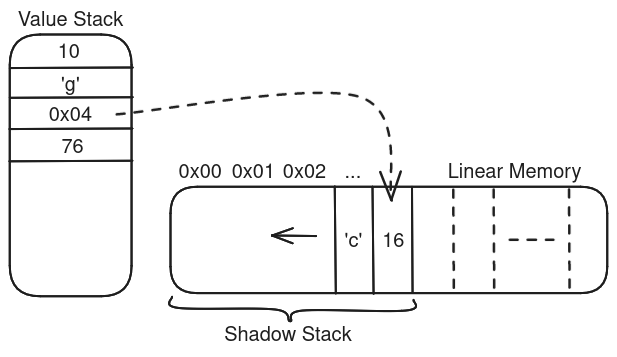
\includegraphics[width=0.5\linewidth]{value_and_shadow_stack.png}
  \caption{Value and Shadow Stack}
  \label{fig:value-shadow-stack}
\end{figure}

Those two stacks are present in the wasm code but when it needs to be translated to the final bytecode the compiler tries to elide every access to the Value Stack allocating everything needed in the registers. Registers are limited though so is impossible to use only them and the native stack of the embedder will be used if needed.

\subsubsection{AOT}

AOT is the standard compilation, all the code is compiled and then executed. Wasmtime is a wasm embedder, it is a stand alone wasm environment but it could be also used as library to create a wasm environment in your bigger application. Wasmtime offer offers this feature, it accept wasm in text or binary format and compiles it to some architecture's bytecode.

\subsubsection{JIT}

JIT is a dynamic compilation where the bytecode si compiled only if it needed, the compiler first need to create an intermediate representation to being able to compile the different parts only if the execution requires to. A really simple example to make is: we have a program that given an input calls function A or B, the JIT then will understand this structure and compile the entry point and only one function between A or B based on the initial input.

Lots of optimizations are already been done in the first phase of compilation, from the High-Level language to WASM, now the main goal is to compile only the required parts to the final bytecode not caring too much about adding optimizations.

Wasmtime is specialized in this type of execution and it makes it really efficient keeping every secure.

\subsubsection{SP} %Single Pass Compile%

A Single Pass compiler is a restriction of AOT compiler, the complexity of the compilation must be O(n) so the wasm bytecode will be scanned through only once. Like every other compilation methods here the trade off si not to create efficient final code but to create the final bytecode as fast as possible.

Wasmer is wasm embedder with a lot of features, in particular they implemented a single pass compiler for all the most important architectures.

\subsubsection{Interpret}
\href{https://github.com/paritytech/Wasmi}{wasmi-spec}

Interpretation is the easiest way to think how to execute wasm, it becomes like any other interpreted language executed by a specialized Virtual Machine. There are multiple ways to interpret code but we will focus on one of the most efficient wasm interpreter, wasmi.

Wasmi is an efficient WebAssembly interpreter with low-overhead and support for embedded environment such as WebAssembly itself. ~\cite{wasmi}

Currently the first wasm bytecode pass produce another stack based bytecode, called WASMI IR, and then this bytecode is interpreted by a Virtual Machine, even with this transpilation it is only 5 time slower then the compilation to native bytecode of the architecture.

\subsection{Security guarantee}

WASM principle aim is to be extremely secure the specifications describe a lot of ways to achieve that feature, but he security guarantee depends mostly on the execution, WebAssembly is designed to be translated into machine code running directly on the host’s hardware. Being so portable wasm can be sent to someone and be executed freely, examples in every browsers. We are running wasm our machines every day and if it would not be so secure then we would had notice a lot of problems.

Executing WASM is potentially vulnerable to side channel attacks on the hardware level ~/cite{wasm-core-spec} and isolation is the only way to make secure the execution. If the embedder translate one on one every instructions then everything can be computed on your computer, but nothing is dangerous if the code has no access to the environment where is executed.

The problem is that a completely isolation makes wasm useless, so there's a way to communicate with the environment or also have access to it, but those features are extremely limited and designed to be secure.

\subsubsection{Linear Memory}
(\href{}{linear-memory})

From WebAssemply you have direct access to raw bytes, but where are allocated those bytes? WASM uses a MemoryObject provided by the embedder to describe the only accessible memory, beside the stack, the linear memory.~\cite{linear-memory}

WASM does not have pointer types, values in the linear memory are accessed as a vector, where the first index of the memory is 0.

Wasm, for security reason that will be explained in next chapters, works in a 32-bit address space, this makes usable only 4GiB of memory. Being the ponear Memory memory unknown to the wasm blob every load or store to the memory is made passing through the embedder that will also do bounds checks to make sure the address is inside the wasm Linear Memory.

\begin{figure}[h]
  \centering
  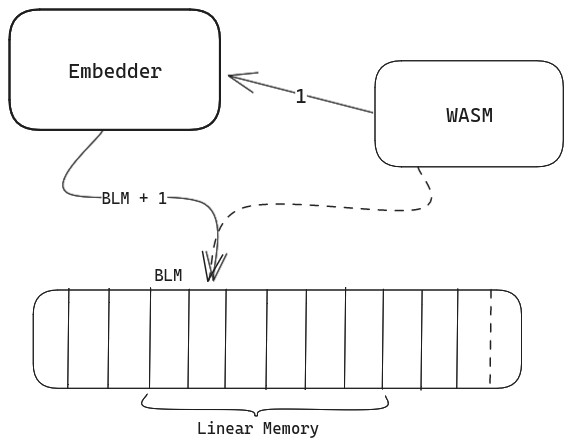
\includegraphics[width=0.5\linewidth]{linear_memory.png}
  \caption{BLM: Base Linear Memory Pointer}
  \label{fig:linear_memory}
\end{figure}

This level of control makes impossible to have memory leak in the environment during the wasm execution because there is a completely memory isolation. ~\cite{linear-memory}

\subsubsection{Communication in a sandboxed environment}

We just described how wasm provides no ambient access to the computing environment in which code is executed ~\cite{wasm-core-spec}, thanks to a mix of wasm design choice and embedder implementation. But how works then the interaction with the environment?

\

Every interaction can be done by a set of functions provided by the embedder and imported in the Wasm module~\cite{wasm-core-spec}, those functions are called Host Functions and allow the WASM code to access to resources, operating system calls or any other type of computation offered by the embedder. Generally the Exports provided by WASM that are usable and callable from the embedder are called Runtime API.

\begin{figure}[h]
  \centering
  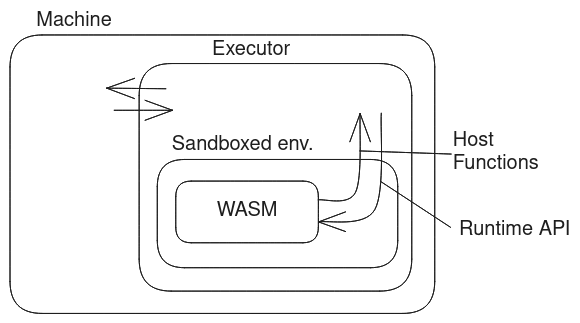
\includegraphics[width=0.5\linewidth]{env_communication.png}
  \caption{Environment communication}
  \label{fig:env-communication}
\end{figure}

\subsubsection{Wasmtime Security guarantee}

Wasmtime is widely used in different environments and one of those is the polkadot ecosystem, precisely wasmtime is used inside substrate. Substrate is a framework to develop blockchains that with some tweaks can become parachains, polkadot itself is a substrate based chain.

Wasmtime main goals is to execute untrusted code in a safe manner.~\cite{wasmtime-book}

Some features that makes executing wasm by wasmtime secure are just inherit by the wasm specifications, some examples are: the callstack is inaccessible, pointers are compiled to offsets into linear memory, there's no undefined behavior and every interaction with the outside world is done through imported and exported functions.~\cite{wasmtime-book}

Wasmtime to those features adds a lot of mitigations to limit issues:
\begin{itemize}
  \item Linear memories by default are preceded with a 2GB guard region
  \item Wasmtime will zero memory used by a WebAssembly instance after it's finished.
  \item Wasmtime uses explicit checks to determine if a WebAssembly function should be considered to stack overflow
  \item The implementation language of wasmtime, Rust, helps catch mistakes when writing Wasmtime itself at compile time
\end{itemize}

\end{document}
